\chapter{Defining Heuristics for Sokoban}
\label{cha:heuristics}

\section{Introduction}
In this chapter we examine which general heuristics are convenient to
the Sokoban domain and how they might be applied. Furthermore we
develop our own domain specific heuristic. These will all be
implemented in the planning application.

\section{General Heuristics}
We are required to implement at least one of the general heuristic
mentioned in \citet{Russell2003GeneralHeuristics}. This heuristic is
meant to be used as a base line of comparison when we implement a more
domain specific heuristic.

There are a number of different, general, ways of building a heuristic
for a given problem. 

\subsection{Relaxing the Sokoban Problem}
In order to relax a STRIPS style problem we can either remove or alter
the pre-conditions and/or effects. This approach has some inherent
challenges that we must overcome. It is also worth remembering that
the developed heuristic \emph{must} be simpler than solving the
original problem in order for this exercise to make any sense.

\subsubsection{Removing Preconditions}

Removing all preconditions in Sokoban 

\subsubsection{SubGoalIndependence}
Another approach is to divide the problem into a number of subproblems. The idea is that when solving the subproblems one at a time, the entire problem will be solved.

\subsection{Implemented heuristics}
In order to find the best heuristics we have implemented many different heuristics. Some are them are very similar while others differ alot. The heuristics can be divided into the categories \textit{The true heuristics} containing the actual heuristics, \textit{Deadlock detection} holding the heuristics which determines whether a deadlock has occurred or not and the \textit{Combiners} which combines a number of heuristics into one.

To get as little code duplication as possible we have our heuristics doing very small things. In order to get a good heuristic we then have to combine the heuristics.

\subsubsection{Combiners}
A \textit{combiner} is a heuristic combining one or more of the heuristics. It has a number of heuristics assigned to it which in the following will be reffered to as its children. When asked for a performance estimate of a given state it will take the performance estimates given by its childrens and combine them into a single performance estimate.
We have implementet two different combiners, a \textit{HeuristicsAdder} and \textit{HeuristicsMultiplier} both sharing a number of methods stored in the abstract class \textit{HeuristicsCombiner}.
%HeuristicsCombiner
\paragraph{HeuristicsAdder}The HeuristicsAdder adds the results of its children. This is useful for when having heuristics used to check for a small part of a gamestate. 
\paragraph{HeuristicsMultiplier}The HeuriscsMultiplier multiplies the results of its children. This is very useful when a heuristic is very critical for the solution. The value of this heuristic can then be multiplied with itself in order to make its performance estimate count much more or to a HeuristicsAdder to make the heurstics in the adder count less.

\subsubsection{The true heuristics}
The true heuristics are the heuristics that does the actual estimation. They estimate how well a given state is depending on the location of the goals, the player and the boxes.

\paragraph{BoxOnGoalHeuristic}The simplest heuristic is the BoxOnGoalHeuristic. It returns the number of boxes not placed on a goal thus making the solutions with boxes put on goals better than those without. It becomes very powerful when multiplying it with an adder containing some of the better heuristics, as the the bonus of having a box on a goal is huge.

\paragraph{SubGoalIndependence}The SubGoalIndependence is a heuristic inspired by the general heuristic mentioned in \citet{Russell2003GeneralHeuristics}. It divides the problem into subproblems looking at only at the player, one box and the goal closest to the box. Then it evaluates the distance from the player to the box and adds it to the distance from the box to the goal. Adding the results of all the boxes an approximation of the number of steps from a given state to the goalstate can be found.

\paragraph{ShortestPathHeuristic}An improvement to the SubGoalIndependence is the ShortestPathHeuristics. It evalutes the distances to all goals from all squares on the board before starting the \astar algorithm. The distances are measured using a BreadthFirst-algorithm that starts in a goal and writes down the distance to the goal in all squares reachable from the goal. This is done for each goal and the result is a map of distances for each goal. An example of such a map can be seen in figure \ref{fig:shortestpathheuristic}.

When running the algorithm the distance from the box to the nearest goal is looked up in these maps and the shortest distance is used. To evaluate the performance estimate in the same way as in the SubGoalIndependence.
\begin{figure}[htp]
	\centering
	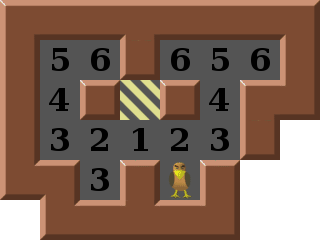
\includegraphics[scale=0.5]{img/src/shortestpathheuristic.png}
	\caption{Distances calculated by the ShortestPathHeuristic}
	\label{fig:shortestpathheuristic}
\end{figure}

\paragraph{AveragePathHeuristic}The AveragePathHeuristic looks much like the ShortestPathHeuristic. Instead of looking at the distance to the nearest goal it takes the average distance to all the goals which are not yet occupied by boxes. In this way a very likely estimation of the number of steps needed to reach the goal state from a given state is estimated.

If it is more important to find a solution quickly than to find a short solution, the distance from the goalstate could be squared. This would make the algorithm weigh the distance higher than the number of steps used and hence make it try the best looking path (even if it does not follow the best possible path) before going back for the second best looking path.

\subsubsection{Deadlock detection}
The heuristics in this category are responsible for finding deadlocks, that is a state where one or more boxes are placed at a spot from which they cannot be moved. When such a state is found an exception is thrown telling the \astar algorithm not to use this state. We have implemented two very simple deadlock detectors, but more and better detectors might be needed for the planner to work better.
\paragraph{Box4x4Heuristic}The Box4x4Heuristic checks every box if they are stuck in a 4x4 block without being on a goal square. If this happens the heuristic will throw an exception telling that this state is not to be used. An example of a state found by this heuristic can be seen on figure \ref{fig:box4x4} on the left.

The heuristic works by for all boxes not standing on goal squares checking if they are placed adjent to boxes or walls making meking them form a 4x4 square. In figure \ref{fig:box4x4} on the right, the algorithm has found a 4x4 square shown by the green square. The red squares indicate that a 4x4 square has not been found in these directions.

\begin{figure}[htp]
	\centering
	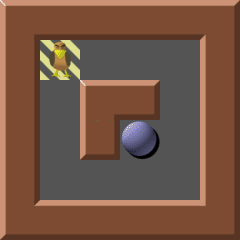
\includegraphics[width=0.3\textwidth]{box4x4}
	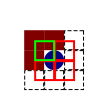
\includegraphics[width=0.3\textwidth]{box4x4detect}
	\caption{Box4x4Heuristic detects this state as a deadlock state.}
	\label{fig:box4x4}
\end{figure}

\paragraph{CornerHeuristic}Another very powerful deadlock detector is the CornerHeuristic. It decides on which squares the boxes will never be allowed, illegal squares, as the boxes will not be able to leave these areas thus making them reach the goal imposible. The illegal squares are found using corners: inner corners indicated by \textit{i} in figure \ref{fig:cornerheuristic} and outer corners indicated by \textit{o}.
\begin{figure}[htp]
	\centering
	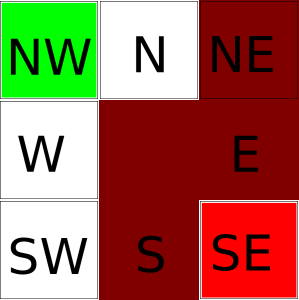
\includegraphics[scale=0.3]{cornerfind}
	\caption{Finding corners}
	\label{fig:cornerheuristic}
\end{figure}
To find the corners the algorithm checks all wall squares. At each wall the algorithm look at the squares located diagonally from the wall, that is the squares NE, NW, SE and SW shown in figure \ref{fig:cornerheuristic}. Using this figure as example the algorithm would check corners as described here:
\begin{itemize}
	\item As the square in NE is a wall it can not be a corner.
	\item The square NW is not a wall and none of the squares N and W are walls. Therefore the square NW is an outer corner.
	\item The squareSW is not a wall but one of the squares S and W is a wall while the other is not. Therefore there is no corner in square SW.
	\item Finally the square SE is not a wall while both of the squares S and E are. This makes the square SE an inner corner.
\end{itemize}

All squares between two inner corners are then seen as illegal squares and these squares will be indicated by \textit{\!}. The inner corner squares are also marked as illegal squares. Squares on the same line as an outer square or a goal is not illegal squares, so when the squares have been marked, the squares on line with goals are unmarked. This is done by checking each goal if they have been marked as an illegal square. If it has been marked, the algorithm finds out in which direction a wall is located and unmarks all fields in the direction ortogonal to this.

In steps the algorithm does the following. The steps is also illustrated in figure \ref{fig:cornerheuristic}.
\begin{itemize}
	\item The map is read
	\item Each corner is found and marked by either \textit{i} or \textit{o}.
	\item All fields between inner corners are marked as illegal squares.
	\item All fields on line with a goal marked as an illegal square are unmarked as boxes are allowed on this line in order to push them onto the goal square.
	\item That leaves all the illegal squares marked.
\end{itemize}

\begin{figure}[htp]
	\centering
	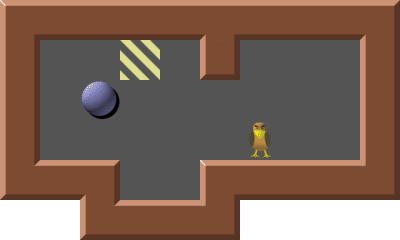
\includegraphics[width=0.33\textwidth]{corner1}
	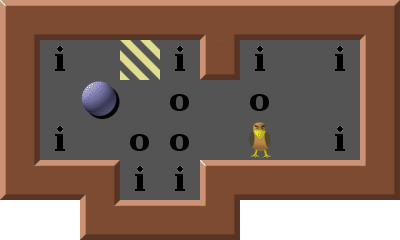
\includegraphics[width=0.33\textwidth]{corner2}
	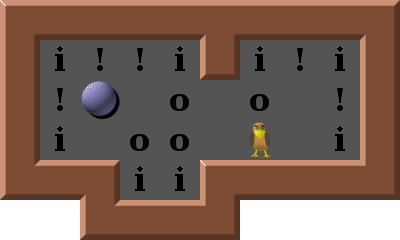
\includegraphics[width=0.33\textwidth]{corner3}
	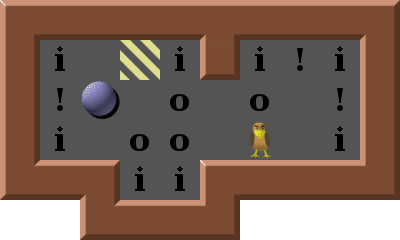
\includegraphics[width=0.33\textwidth]{corner4}
	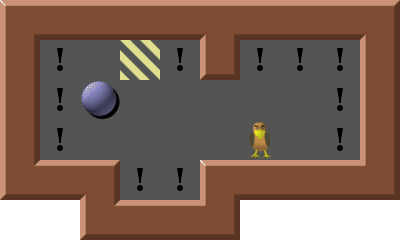
\includegraphics[width=0.33\textwidth]{corner5}
	\caption{CornerHeuristic in steps}
	\label{fig:cornerheuristic}
\end{figure}










